\documentclass[xelatex,aspectratio=169]{beamer}

\hfuzz=10pt
\vfuzz=10pt

% Theme
\usetheme{htw}
\setbeamertemplate{navigation symbols}{}
\setbeamertemplate{theorems}[numbered]
\setbeamercovered{transparent}

%\logo{
\includegraphics[height=0.5cm]{HTWD_color.png}}

% Packages
\usepackage{polyglossia}
\setmainlanguage{german}
\setotherlanguage{english}

\usepackage[bigfiles]{pdfbase}
\ExplSyntaxOn
\NewDocumentCommand\embedvideo{smm}{
\group_begin:
\leavevmode
\tl_if_exist:cTF{file_\file_mdfive_hash:n{#3}}{
  \tl_set_eq:Nc\video{file_\file_mdfive_hash:n{#3}}
}{
  \IfFileExists{#3}{}{\GenericError{}{File~`#3'~not~found}{}{}}
  \pbs_pdfobj:nnn{}{fstream}{{}{#3}}
  \pbs_pdfobj:nnn{}{dict}{
    /Type/Filespec/F~(#3)/UF~(#3)
    /EF~<</F~\pbs_pdflastobj:>>
  }
  \tl_set:Nx\video{\pbs_pdflastobj:}
  \tl_gset_eq:cN{file_\file_mdfive_hash:n{#3}}\video
}
%
\pbs_pdfobj:nnn{}{dict}{
  /Type/RichMediaInstance/Subtype/Video
  /Asset~\video
  /Params~<</FlashVars (
  source=#3&
  skin=SkinOverAllNoFullNoCaption.swf&
  skinAutoHide=true&
  skinBackgroundColor=0x5F5F5F&
  skinBackgroundAlpha=0.75
  )>>
}
%
\pbs_pdfobj:nnn{}{dict}{
/Type/RichMediaConfiguration/Subtype/Video
/Instances~[\pbs_pdflastobj:]
}
%
\pbs_pdfobj:nnn{}{dict}{
/Type/RichMediaContent
/Assets~<<
/Names~[(#3)~\video]
>>
/Configurations~[\pbs_pdflastobj:]
}
\tl_set:Nx\rmcontent{\pbs_pdflastobj:}
%
\pbs_pdfobj:nnn{}{dict}{
  /Activation~<<
  /Condition/\IfBooleanTF{#1}{PV}{XA}
  /Presentation~<</Style/Embedded>>
  >>
  /Deactivation~<</Condition/PI>>
}
%
\hbox_set:Nn\l_tmpa_box{#2}
\tl_set:Nx\l_box_wd_tl{\dim_use:N\box_wd:N\l_tmpa_box}
\tl_set:Nx\l_box_ht_tl{\dim_use:N\box_ht:N\l_tmpa_box}
\tl_set:Nx\l_box_dp_tl{\dim_use:N\box_dp:N\l_tmpa_box}
\pbs_pdfxform:nnnnn{1}{1}{}{}{\l_tmpa_box}
%
\pbs_pdfannot:nnnn{\l_box_wd_tl}{\l_box_ht_tl}{\l_box_dp_tl}{
  /Subtype/RichMedia
  /BS~<</W~0/S/S>>
  /Contents~(embedded~video~file:#3)
  /NM~(rma:#3)
  /AP~<</N~\pbs_pdflastxform:>>
  /RichMediaSettings~\pbs_pdflastobj:
  /RichMediaContent~\rmcontent
}
\phantom{#2}
\group_end:
}
\ExplSyntaxOff


\usepackage{graphicx}
\usepackage[export]{adjustbox}
\usepackage{animate}
%\usepackage[dvipdfmx]{movie15_dvipdfmx}
\usepackage{media9}
\usepackage{tabularx}
\usepackage{colortbl}
\usepackage{booktabs}
\usepackage{makecell}
\usepackage{ltablex}
\usepackage{array}
\usepackage{multirow}
\usepackage{amsmath}
\usepackage{amsthm}
%\renewcommand{\arraystretch}{1.5}
\newcolumntype{L}[1]{>{\raggedright\let\newline\\\arraybackslash\hspace{0pt}}p{#1}}
\newcolumntype{C}[1]{>{\centering\let\newline\\\arraybackslash\hspace{0pt}}p{#1}}
\newcolumntype{R}[1]{>{\raggedleft\let\newline\\\arraybackslash\hspace{0pt}}p{#1}}
%\renewcommand\thesatz{\arabic{section}.\arabic{theorem}}
\makeatletter
\@addtoreset{theorem}{lecture}
\makeatother

\newtheorem{satz}{Satz}[section]
\newtheorem{lem}{Lemma}[section]
\newtheorem{beh}{Behauptung}[section]
\newtheorem{define}{Definition}[section]
\numberwithin{equation}{section}
\usepackage{ragged2e}
\usepackage{etoolbox}

\usepackage{color}
\usepackage{colortbl}
\definecolor{hellgrau}{rgb}{0.85,0.85,0.85}
\definecolor{hellrot}{rgb}{1,0.7,0.7}

\usepackage{tikz}
\usetikzlibrary{shapes,arrows.meta,calc,arrows,positioning,patterns,tikzmark}
%\usepackage{tikz-uml}
\usepackage{pgfplots}  % for elliptic curves (part 8)
\pgfplotsset{compat=1.18}
\usepackage{pgffor}
\usepackage{pgfmath-xfp}
\tikzset{>=latex}
\tikzset{
  invisible/.style={opacity=0},
  visible on/.style={alt={#1{}{invisible}}},
  alt/.code args={<#1>#2#3}{%
      \alt<#1>{\pgfkeysalso{#2}}{\pgfkeysalso{#3}} % \pgfkeysalso doesn't change the path
    },
}

\usepackage{paralist}

\usepackage{url}
\def\UrlBreaks{\do\/\do-}
\PassOptionsToPackage{hyphens}{url}\usepackage{hyperref}

\usepackage[normalem]{ulem} % gestrichelte Unterstreichung (\dashuline{})
\usepackage{cancel}

\makeatletter
\renewcommand{\itemize}[1][]{%
  \beamer@ifempty{#1}{}{\def\beamer@defaultospec{#1}}%
  \ifnum \@itemdepth >2\relax\@toodeep\else
    \advance\@itemdepth\@ne
    \beamer@computepref\@itemdepth% sets \beameritemnestingprefix
    \usebeamerfont{itemize/enumerate \beameritemnestingprefix body}%
    \usebeamercolor[fg]{itemize/enumerate \beameritemnestingprefix body}%
    \usebeamertemplate{itemize/enumerate \beameritemnestingprefix body begin}%
    \list
    {\usebeamertemplate{itemize \beameritemnestingprefix item}}
    {\def\makelabel##1{%
        {%
            \hss\llap{{%
                  \usebeamerfont*{itemize \beameritemnestingprefix item}%
                  \usebeamercolor[fg]{itemize \beameritemnestingprefix item}##1}}%
          }%
      }%
    }
  \fi%
  \beamer@cramped%
  \justifying% NEW
  %\raggedright% ORIGINAL
  \beamer@firstlineitemizeunskip%
}
\makeatother

\apptocmd{\frame}{}{\justifying}{}

\renewcommand\theadfont{\bfseries\sffamily}
\usepackage{ragged2e}
\usepackage{newpxtext}

\setsansfont{texgyreheros}[
  Scale=MatchLowercase,
  UprightFont=*-regular,
  BoldFont=*-bold,
  ItalicFont=*-italic,
  BoldItalicFont=*-bolditalic,
]

% Title
\usepackage[usetransparent=false]{svg}
% Import references
\usepackage[backend=biber,style=numeric,sorting=none]{biblatex}
\addbibresource{references.bib}

%\AtBeginSection[]{
%  \begin{frame}
%    \vfill
%    \centering
%    \begin{beamercolorbox}[sep=8pt,center,shadow=true,rounded=true]{title}
%      \usebeamerfont{title}\thesection.~\secname\par%
%    \end{beamercolorbox}
%    \vfill
%  \end{frame}
%}

\makeatletter
\newenvironment{noheadline}{
  \setbeamertemplate{headline}{}
  \addtobeamertemplate{frametitle}{\vspace*{-0.9\baselineskip}}{}
}{}
\makeatother


\usepackage{xcolor}
\usepackage{algorithm}
\usepackage[linesnumbered,ruled,lined,commentsnumbered,algo2e,ngerman,ngermankw]{algorithm2e}
\usepackage{algorithmic}
\usepackage{caption}
\usepackage[newfloat]{minted}
\captionsetup[listing]{position=top}
\definecolor{mintedbg}{HTML}{282828}
\setminted{
  breaklines=true,
  bgcolor=mintedbg,
  style=monokai,
  formatcom=\color{white}
}
\usepackage{etoolbox}
\makeatletter
% replace \medskip before and after the box with nothing, i.e., remove it
\patchcmd{\minted@colorbg}{\medskip}{}{}{}
\patchcmd{\endminted@colorbg}{\medskip}{}{}{}
\makeatother

\renewcommand{\theFancyVerbLine}{\textcolor{black}{\arabic{FancyVerbLine}}}

\usepackage{pifont}
\newcommand{\cmark}{\ding{51}}%
\newcommand{\xmark}{\ding{55}}%

\newenvironment{changemargin}[2]{%
  \begin{list}{}{%
      \setlength{\topsep}{0pt}%
      \setlength{\leftmargin}{#1}%
      \setlength{\rightmargin}{#2}%
      \setlength{\listparindent}{\parindent}%
      \setlength{\itemindent}{\parindent}%
      \setlength{\parsep}{\parskip}%
    }%
    \item[]}{\end{list}}


\usepackage{csquotes}

% Title
\title{Aussagenlogik}
\author{Prof. Dr. Lukas Iffländer}
\institute{HTW Dresden}
\date{}
\usepackage{svg}

% Begin document
\begin{document}

% Title slide
\begin{frame}
  \titlepage
\end{frame}

\section{Aussagen}

\begin{frame}{Aussagen}
  \begin{block}{Definition}
    Aussagen sind formulierte
    \begin{itemize}
      \item numerische Bedingungen, zum Beispiel $x<5$
      \item Relationen zwischen Variablenwerten, wie \mintinline{python}|a[i] < a[i+1]$|
      \item berechnete Aussagen, wie z.B. \mintinline{python}|schaltjahr(j)|
      \item Wissensrepräsentierende Annahmen, wie zum Beispiel
            \begin{itemize}
              \item R1 für Reifen 1 intakt
              \item D1 für Reifen 1 defekt (es gilt $D1 \implies \mbox{NICHT}(R1)$)
            \end{itemize}
    \end{itemize}
  \end{block}
  \begin{alertblock}{}
    Aussagen können erfüllt und damit wahr sein oder nicht erfüllt und damit falsch sein.
  \end{alertblock}
\end{frame}

\begin{frame}{Aussagen}
  \begin{block}{Eigenschaften}
    Aussagen \ldots
    \begin{itemize}
      \item können den Steuerfluss eines Programms beeinflussen
      \item können logisch verknüpft werden und ergeben neue Aussagen
      \item repräsentieren Wissen in ihrer logischen Verknüpfung
      \item sind möglicherweise Eingabe oder Ausgabe von Programmen und werden durch Programme berechnet
    \end{itemize}
  \end{block}
\end{frame}

\begin{frame}{Wissensrepräsentation}{Beispiel: LKW}
  \begin{columns}
    \begin{column}{0.5\textwidth}
      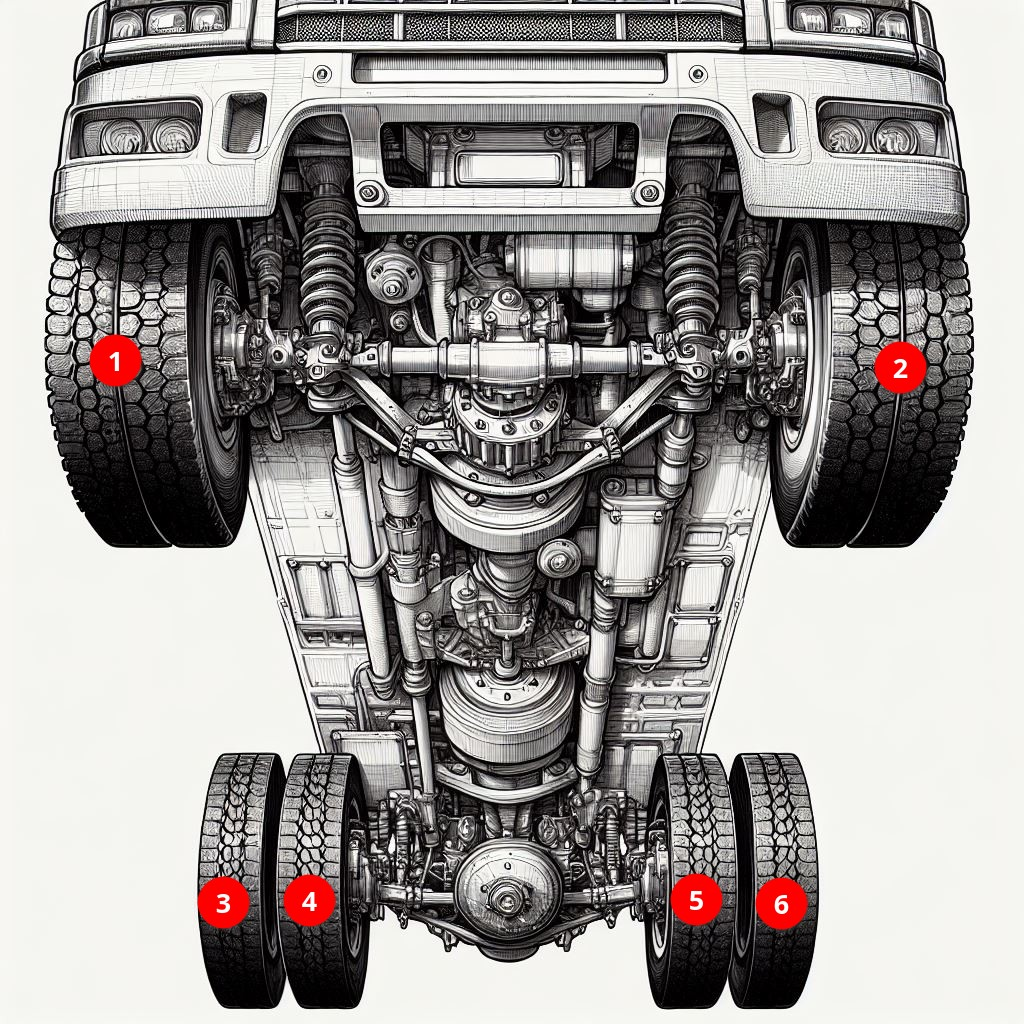
\includegraphics[width=\textwidth]{img/lkw_bottom.jpg}
    \end{column}
    \begin{column}{0.5\textwidth}
      \(R_i\) für Reifen i intakt \\
      \(D_i\) für Reifen i defekt

      Expertenwissen:

      \begin{itemize}
        \item \(D_i \implies \mbox{NICHT}(R_i)\)
        \item FahrzeugOK = R1 UND R2 UND R3 UND R4 UND R5 und R6
        \item NichtFahrbereit = D1 oder D2 oder (D3 und D4) oder (D5 und D6)
      \end{itemize}
    \end{column}
  \end{columns}
\end{frame}

\section{Aussagenlogik}

\begin{frame}{Aussagenlogik}
  \begin{columns}
    \begin{column}{0.65\textwidth}
      \begin{block}{Herkunft}
        Mathematische Grundlagen durch die Boolesche Algebra als Logik-Kalkül (George Boole, 1847)
      \end{block}
      \begin{block}{Anwendungungen}
        \begin{itemize}
          \item \textbf{Aussagenlogik} mit 0 als falsch und 1 als wahr
          \item Mengenlehre
          \item Schaltalgebra mit 0 (Schaltzustand AUS bzw Spannung niedrig) und 1 (Schaltzustand EIN bzw Spannung hoch)
        \end{itemize}

      \end{block}
    \end{column}
    \begin{column}{0.35\textwidth}
      \centering George Boole (1815-1864)
      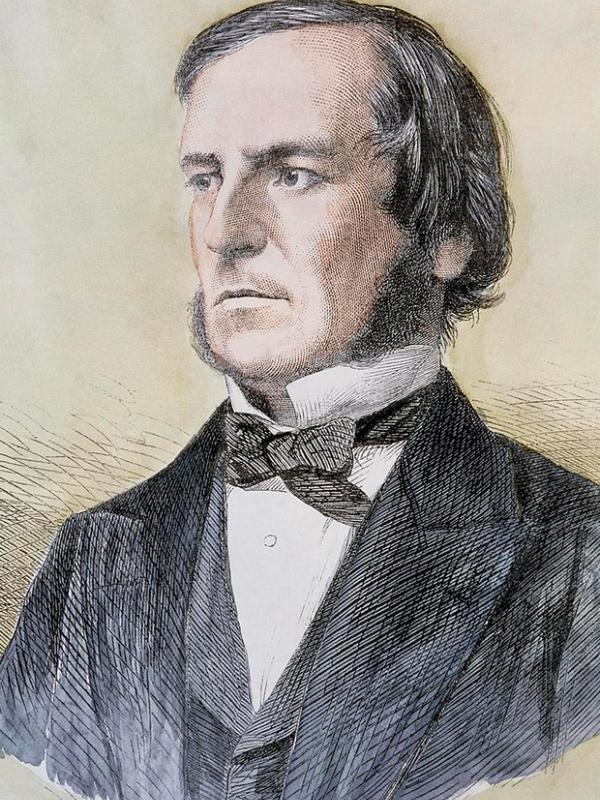
\includegraphics[height=.7\textheight]{img/George_Boole.jpg}
    \end{column}
  \end{columns}
\end{frame}

\begin{frame}{Andere Logiken}
  \begin{columns}
    \begin{column}{0.5\textwidth}
      \begin{exampleblock}{Prädikatenlogik (Erweiterung der Aussagenlogik)}
        \begin{align*}
          \exists x \in \mathbb{N} & : x = \left|x\right| \\
          \forall x \in \mathbb{N} & : x - 1 < x
        \end{align*}
      \end{exampleblock}
      \begin{exampleblock}{Fuzzy Logik}
        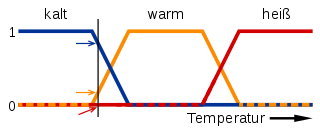
\includegraphics[width=\textwidth]{img/fuzzy_logic.png}
      \end{exampleblock}
    \end{column}
    \begin{column}{0.5\textwidth}
      \begin{exampleblock}{Temporale Logik}
        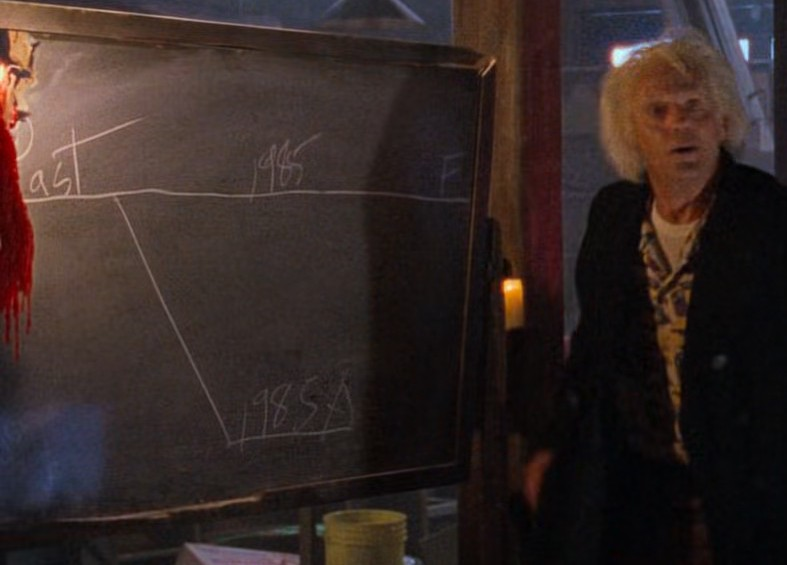
\includegraphics[width=\textwidth]{img/temporal_logic_doc_brown.jpg}
      \end{exampleblock}
    \end{column}
  \end{columns}
\end{frame}

\begin{frame}{Logik-Kalkül (George Boole, 1847)}
  \begin{definition}
    Eine Menge $B$ von Elementen, über der zwei Operationen (\(+\) und (\(\cdot\)) definiert sind, ist genau dann Boolesche Algebra \( B; +, \cdot\) wenn für beliebige Elemente \(a\), \(b\), \(c\) aus \(B\) die folgenden Axiome gelten:
    \begin{itemize}
      \item \textbf{Kommutativgesetz}:
            \begin{itemize}
              \item \(a + b = b + a\)
              \item \(a \cdot b = b \cdot a\)
            \end{itemize}
      \item \textbf{Assoziativgesetz}:
            \begin{itemize}
              \item \(a + (b + c) = (a + b) + c\)
              \item \(a \cdot (b \cdot c) = (a \cdot b) \cdot c\)
            \end{itemize}
      \item \textbf{Distributivgesetz}:
            \(a + (b \cdot c) = (a + b) \cdot (a + c)\)
      \item \textbf{Identitätsgesetz}:
            \(a + 0 = a\) und \(a \cdot 1 = a\)
      \item \textbf{Negationsgesetz}:
            \(a + 1 = 1\) und \(a \cdot 0 = 0\)
      \item \textbf{Idempotenzgesetz}:
            \(a + a = a\) und \(a \cdot a = a\)
            %\item $x^2=x$ und $x+x=x$
    \end{itemize}
  \end{definition}
\end{frame}

\begin{frame}{Aussagenlogik}{Als Boolesche Algebra}
  \begin{definition}
    Die Aussagenlogik ist eine Boolesche Algebra. Es gelten damit die Gesetze der Booleschen Algebra.
  \end{definition}

  \begin{block}{Werte}
    \centering
    \begin{tabular}{ccc}
      \toprule
      \textbf{Wert} & \multicolumn{2}{c}{\textbf{Bezeichnungen}}         \\
      \midrule
      0             & Falsch                                     & False \\
      1             & Wahr                                       & True  \\
      \bottomrule
    \end{tabular}
  \end{block}
\end{frame}

\begin{frame}{Aussagenlogik}{Operationen}
  \begin{block}{Operationen}
    \centering
    \begin{tabular}{lcccc}
      \toprule
      \multicolumn{3}{c}{\textbf{Bezeichnungen}} & \textbf{Symbol} & \textbf{Python-Operator}                                            \\
      \midrule
      Konjunktion                                & \textbf{UND}    & \textbf{AND}             & \(\land\)                          & and \\
      Disjunktion                                & \textbf{ODER}   & \textbf{OR}              & \(\lor\)                           & or  \\
      Negation                                   & \textbf{NICHT}  & \textbf{NOT}             & \(\lnot\) oder \(\overline{WERT}\) & not \\
      \toprule
    \end{tabular}
  \end{block}
\end{frame}

\begin{frame}{Aussagenlogik}{Rechenregeln}
  Defination der Operationen Konjunktion, Disjunktion und Negation über Wahrheitstafeln:
  \begin{columns}[onlytextwidth]
    \begin{column}{0.48\textwidth}
      \begin{block}{Konjunktion}
        \centering\small
        \begin{tabular}{ccc}
          \toprule
          $A$ & $B$ & $A \land B$ \\
          \midrule
          0   & 0   & 0           \\
          0   & 1   & 0           \\
          1   & 0   & 0           \\
          1   & 1   & 1           \\
          \bottomrule
        \end{tabular}
      \end{block}
    \end{column}
    \begin{column}{0.48\textwidth}
      \begin{block}{Disjunktion}
        \centering\small
        \begin{tabular}{ccc}
          \toprule
          $A$ & $B$ & $A \lor B $ \\
          \midrule
          0   & 0   & 0           \\
          0   & 1   & 1           \\
          1   & 0   & 1           \\
          1   & 1   & 1           \\
          \bottomrule
        \end{tabular}
      \end{block}
    \end{column}
  \end{columns}
  \begin{block}{Negation}
    \centering\small
    \begin{tabular}{cc}
      \toprule
      $A$ & $\lnot A$ \\
      \midrule
      0   & 1         \\
      1   & 0         \\
      \bottomrule
    \end{tabular}
  \end{block}
\end{frame}

\begin{frame}{Logik in verschiedenen Systemen}
  \vspace{-1em}
  \begin{columns}
    \begin{column}{0.5\textwidth}
      \begin{block}{Aussagenlogik für Programme}
        \inputminted[firstline=5,lastline=8]{python}{src/logik_example.py}
      \end{block}
    \end{column}
    \begin{column}{0.5\textwidth}
      \begin{block}{Schaltalgerba}
        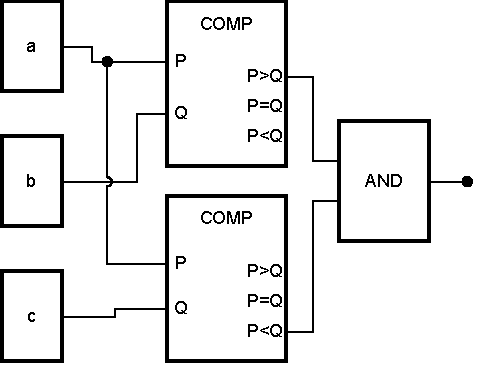
\includegraphics[width=\textwidth]{fig/logik_schaltalgebra.pdf}
      \end{block}
    \end{column}
  \end{columns}
  \vspace{1em}
\end{frame}

\begin{frame}{Bedingungsausdrücke}
  Einzelne Aussagen können Bedingungsausdrücke sein:
  \begin{itemize}
    \item[~] Aussage \texttt{kalt}: \(\mbox{temperatur} < 10\)
    \item[~] Aussage \texttt{zu\_schnell}: \(V > 100\)
  \end{itemize}

  Bedingungsausdrücke werden durch aussagelogische Operationen verknüpft:

  \begin{exampleblock}{Beispiel}
    \begin{align*}
      \lnot \left( zahl < 0 \right) & \land \lnot (zahl > 64) \\
      zahl \geq 0                   & \land zahl \leq 64      \\
      \lnot ( zahl < 0              & \lor zahl > 64 )
    \end{align*}
    \only<2->{Alle drei Ausdrücke sind gleichwertig. zahl ist zwischen 0 und 64.}
  \end{exampleblock}

\end{frame}

\begin{frame}{Aussagenlogik}{Eigenschaften}
  \centering Eigenschaften als Anwendung des Logik-Kalküls
  \begin{columns}
    \begin{column}{0.5\textwidth}
      \begin{block}{Kommutativität}
        \vspace{-\baselineskip}
        \begin{align*}
          A \land B & \equiv B \land A \\
          A \lor B  & \equiv B \lor A
        \end{align*}
      \end{block}

      \begin{block}{Neutrales Element}
        \vspace{-\baselineskip}
        \begin{align*}
          A \land \texttt{WAHR}  & \equiv A \\
          A \lor \texttt{FALSCH} & \equiv A
        \end{align*}
      \end{block}
    \end{column}
    \begin{column}{0.5\textwidth}
      \begin{block}{Distributivität}
        \vspace{-\baselineskip}
        \begin{align*}
          A \land (B \lor C) & \equiv (A \land B) \lor (A \land C) \\
          A \lor (B \land C) & \equiv (A \lor B) \land (A \lor C)
        \end{align*}
      \end{block}
      \begin{block}{Komplementäres Element}
        \vspace{-\baselineskip}
        \begin{align*}
          A \land \lnot A & \equiv \texttt{FALSCH} \\
          A \lor \lnot A  & \equiv \texttt{WAHR}
        \end{align*}
      \end{block}
    \end{column}
  \end{columns}
  \begin{exampleblock}{}
    \( \equiv \) bedeutet, dass linke und rechte Seite logisch gleichwertig sind und ineinander umgeformt werden können.
  \end{exampleblock}
\end{frame}

\begin{frame}{Aussagenlogik}{Eigenschaften}
  \begin{block}{Verkettung von Operationen gleichwertiger Art (Assoziativität)}
    \vspace{-\baselineskip}
    \begin{align*}
      (A \land B) \land C & \equiv A \land (B \land C) \longleftrightarrow A \land B \land C \\
      (A \lor B) \lor C   & \equiv A \lor (B \lor C) \longleftrightarrow A \lor B \lor C
    \end{align*}
  \end{block}
  \begin{block}{Verkettung von Operationen ungleicher Art (Distributivität)}
    \vspace{-\baselineskip}
    \begin{align*}
      (A \land B) \lor C & \equiv (A \lor B) \land (A \lor C)  \\
      A \land (B \lor C) & \equiv (A \land B) \lor (A \land C) \\
      \\
      (A \lor B) \land C & \equiv (A \land B) \lor (A \land C) \\
      A \lor (B \land C) & \equiv (A \lor B) \land (A \lor C)
    \end{align*}
  \end{block}
\end{frame}

\begin{frame}{Aussagenlogik}{Eigenschaften}
  \begin{block}{Dualitätsprinzip}
    Für eine Regel gibt es immer eine weitere (gespiegelte) Regel, die durch Tauschen der Operation UND mit ODER und umgekehrt, sowie Austausch von WAHR und FALSCH entsteht. Zusätzlich gilt, dass jede aussagelogische Identität eine duale Identität hat.
    \vspace{-\baselineskip}
    \begin{align*}
      (A \land\tikzmark{aland_1} B) \lor\tikzmark{alor_2} C & \equiv (A \lor\tikzmark{alor_3} C) \land\tikzmark{aland_4} (B \lor\tikzmark{alor_5} C)   \\
      \\
      (A \lor\tikzmark{blor_1} B) \land\tikzmark{bland_2} C & \equiv (A \land\tikzmark{bland_3} C) \lor\tikzmark{blor_4} (B \land\tikzmark{bland_5} C) \\
      \\
      A \land\tikzmark{cland_1} \lnot A                     & \equiv \mbox{FAL\tikzmark{cfalse}SCH}                                                    \\
      \\
      A \lor\tikzmark{dlor_1} \lnot A                       & \equiv \mbox{WA\tikzmark{dtrue}HR}
    \end{align*}



    \begin{tikzpicture}[remember picture]
      \draw[overlay, <->, line width=1.5pt] ([yshift=-.2\baselineskip,xshift=-.7em]pic cs:aland_1) to ([yshift=.7\baselineskip,xshift=-.7em]pic cs:blor_1);
      \draw[overlay, <->, line width=1.5pt] ([yshift=-.2\baselineskip,xshift=-.7em]pic cs:alor_2) to ([yshift=.7\baselineskip,xshift=-.7em]pic cs:bland_2);
      \draw[overlay, <->, line width=1.5pt] ([yshift=-.2\baselineskip,xshift=-.7em]pic cs:alor_3) to ([yshift=.7\baselineskip,xshift=-.7em]pic cs:bland_3);
      \draw[overlay, <->, line width=1.5pt] ([yshift=-.2\baselineskip,xshift=-.7em]pic cs:aland_4) to ([yshift=.7\baselineskip,xshift=-.7em]pic cs:blor_4);
      \draw[overlay, <->, line width=1.5pt] ([yshift=-.2\baselineskip,xshift=-.7em]pic cs:alor_5) to ([yshift=.7\baselineskip,xshift=-.7em]pic cs:bland_5);

      \draw[overlay, <->, line width=1.5pt] ([yshift=-.2\baselineskip,xshift=-.7em]pic cs:cland_1) to ([yshift=.7\baselineskip,xshift=-.7em]pic cs:dlor_1);
      \draw[overlay, <->, line width=1.5pt] ([yshift=-.2\baselineskip,xshift=-.7em]pic cs:cfalse) to ([yshift=.7\baselineskip,xshift=-.5em]pic cs:dtrue);
    \end{tikzpicture}
    \vspace{-\baselineskip}
  \end{block}
\end{frame}

\begin{frame}{Aussagenlogik}{Regeln}
  \begin{block}{Verkettung unterschiedlicher Operationen}
    \[ (A \land B) \lor C \not\equiv A \land (B \lor C) \]

    Das bedeutet, dass sich für ausgewählte Werte von \(A\), \(B\) und \(C\) unterschiedliche Ergebnisse der Ausdrücke ergeben können.
  \end{block}
  \begin{block}{Klammerung}
    Klammerung kann Ausführungsreihenfolge beeinflussen.

    Beispiel:
    \[ (\mbox{Kaffee} \land \mbox{Milch}) \lor \mbox{Tee} \not\equiv \mbox{Kaffee} \land (\mbox{Milch} \lor \mbox{Tee}) \]
  \end{block}
\end{frame}

\begin{frame}{Aussagenlogik}{Regeln}
  \begin{block}{De Morgan'sche Regel}

    \begin{align*}
      \lnot (A \land B) & \equiv \lnot A \lor \lnot B  \\
      \lnot (A \lor B)  & \equiv \lnot A \land \lnot B
    \end{align*}
  \end{block}
  \begin{exampleblock}{Beispiel}
    \begin{align*}
      \lnot (\mbox{schön} \land \mbox{reich}) \equiv \lnot \mbox{schön} \lor \lnot \mbox{reich} \\
      \lnot (\mbox{regen} \lor \mbox{schnee}) \equiv \lnot \mbox{regen} \land \lnot \mbox{schnee}
    \end{align*}

  \end{exampleblock}
\end{frame}

\begin{frame}{Aussagenlogik}{Regeln}
  \begin{block}{Negation der Negation}

    \begin{align*}
      \lnot (\lnot A) & \equiv A
    \end{align*}
  \end{block}
\end{frame}

\begin{frame}{Aussagenlogik}{XOR}
  \begin{block}{Exklusives ODER (XOR)}
    \centering
    \begin{tabular}{ccc}
      \toprule
      $A$ & $B$ & $A \oplus B$ \\
      \midrule
      0   & 0   & 0            \\
      0   & 1   & 1            \\
      1   & 0   & 1            \\
      1   & 1   & 0            \\
      \bottomrule
    \end{tabular}
  \end{block}

\end{frame}

\begin{frame}{Aussagenlogik}{Operatorprioritäten}
  \begin{columns}
    \begin{column}{0.5\textwidth}
      \begin{block}{Regel}
        \tikzmark{highest}Höchste Priorität -- Ausführung immer vor den anderen Operationen

        \begin{enumerate}
          \item Auflösung von Zahlenrelationen
          \item Negation
          \item Konjunktion
          \item Disjunktion
          \item Folgerung
          \item Äquivalenz
        \end{enumerate}

        \tikzmark{lowest}Niedrigste Priorität -- Ausführung immer nach den anderen Operationen

        \begin{tikzpicture}[remember picture]
          \draw[overlay, ->, line width=1.5pt] ([yshift=-1.2\baselineskip,xshift=.2em]pic cs:highest) to ([yshift=.7\baselineskip,xshift=.2em]pic cs:lowest);
        \end{tikzpicture}

      \end{block}
    \end{column}
    \begin{column}{0.5\textwidth}
      \begin{exampleblock}{Beispiel}
        \small
        \[ \overbrace{\underbrace{\overbrace{\lnot (\underbrace{x < 0}_{1.})}^{2.} \land \overbrace{\lnot (\underbrace{y < 0}_{1.})}^{2.}}_{3.} \lor \underbrace{L > 4}_{1.}}^{4.} \]
      \end{exampleblock}
    \end{column}
  \end{columns}

\end{frame}

\begin{frame}{Aussagenlogik}{Belegungen}
  \[ F \left(a, b, c, d\right) \equiv a \land b \lor b \land c \lor c \land d \]

  \begin{definition}
    Jede Festlegung aller Variablen bildet eine Belegung.
  \end{definition}

  \begin{exampleblock}{Beispiel}
    \begin{itemize}
      \item \( a = \text{wahr}, b = \text{wahr}, c = \text{wahr}, d = \text{wahr} \)
      \item \( a = \text{wahr}, b = \text{wahr}, c = \text{wahr}, d = \text{falsch} \)
      \item \( a = \text{falsch}, b = \text{falsch}, c = \text{falsch}, d = \text{falsch} \)
    \end{itemize}
  \end{exampleblock}

  \begin{block}{Anzahl möglicher Belegungen}
    \begin{itemize}
      \item \( 2^n \) Belegungen
      \item \( n \) ist die Anzahl der Variablen
    \end{itemize}
  \end{block}

\end{frame}

\begin{frame}{Aussagen und Relationen}
  \begin{columns}[T]
    \begin{column}{0.5\textwidth}
      \begin{block}{Aussagenlogik}
        \begin{itemize}
          \item Binäre Variablen und Konstanten können nur zwei Werte annehmen: wahr oder falsch.
          \item Grundoperationen: \( \land, \tikzmark{basicoperations}\lor, \lnot \)
        \end{itemize}
      \end{block}
    \end{column}
    \begin{column}{0.5\textwidth}
      \begin{block}{Numerisches Rechnen mit Zahlenwerten}
        \begin{itemize}
          \item Zahlenvariablen und Konstanten mit (un)endlich vielen Werten
          \item Grundoperationen: \( +, -, \times, / \)
          \item Relationen (Teil der Operationen): \tikzmark{relations}\( <, \leq, =, \neq, \geq, > \) sind erfüllt oder nicht erfüllt und bilden auf Aussagen ab
        \end{itemize}
      \end{block}
    \end{column}
    \begin{tikzpicture}[remember picture, overlay]
      \node[below=1.1cm, text width=5cm] at (pic cs:basicoperations) {Relationen zwischen numerischen Werten und Konstanten gehen als Teile in aussagelogische Ausdrücke ein.};
      \draw[<-, line width=3pt] ([yshift=-\baselineskip] pic cs:basicoperations) to[bend right] ([xshift=-3em]pic cs:relations);
    \end{tikzpicture}
  \end{columns}
\end{frame}

\begin{frame}{Aussagen und Relationen}
  \begin{exampleblock}{Beispiele}
    \vspace{-\baselineskip}
    \begin{align*}
      t > 80                   & \lor P > 3.8                   \\
      \mbox{alter} < 18        & \land \mbox{gewicht} > 100     \\
      \mbox{abschlussnote} = 1 & \land \mbox{studiendauer} < 10 \\
      \lnot (\mbox{anzahl}     & > 100)
    \end{align*}
  \end{exampleblock}
\end{frame}

\begin{frame}{Aussagen und Relationen}{Negation bezüglich Vergleichsoperationen}
  \begin{columns}
    \begin{column}{0.3\textwidth}
      \centering
      \begin{tabular}{lc}
        \toprule
        \textbf{Variable} & \textbf{Relation} \\
        \midrule
        $a$               & $x < 5$           \\
        $\lnot a$         & $x \geq 5$        \\
        \\
        $b$               & $r > s$           \\
        $\lnot b$         & $r \leq s$        \\
        \\
        $c$               & $i = j$           \\
        $\lnot c$         & $i \neq j$        \\
        \bottomrule
      \end{tabular}
    \end{column}
    \begin{column}{0.7\textwidth}
      \begin{block}{De Morgansches Gesetz}
        \[ a \land b \equiv \lnot (\lnot a \lor \lnot b) \]

      \end{block}

      \begin{exampleblock}{Anwendung}
        \centering
        \( a \land b \land c \)

        in einer Form als

        \( x < 5 \land r > s \land i = j \)

        kann umgeformt werden zu

        \( \lnot ( \lnot a  \lor \lnot b \lor \lnot c) \)

        und weiter zu

        \( \lnot (x \geq 5 \lor r \leq s \lor i \neq j) \)
      \end{exampleblock}
    \end{column}
  \end{columns}

\end{frame}

\begin{frame}[t]{Wahrheitstabelle}
  \vspace{-\baselineskip}
  \begin{center}
    \begin{tabular}{rrrr}
      \toprule
      \textbf{a}           & \textbf{b} & \textbf{c}           & \textbf{Logikfunktion}   \\
                           &            &                      & $y = f (a,b,c)$          \\

      \midrule
      \tikzmark{firstrow}0 & 0          & 0                    & 0\tikzmark{firstrowlast} \\
      0                    & 0          & 1                    & 1                        \\
      0                    & 1          & 0                    & 1                        \\
      0                    & 1          & 1                    & 0                        \\
      1                    & 0          & 0                    & 0                        \\
      1                    & 0          & 1                    & 1                        \\
      1                    & 1          & 0                    & 0                        \\
      \tikzmark{lastrow1}1 & 1          & 1\tikzmark{lastrow3} & 1\tikzmark{lastrowlast}  \\
      \bottomrule
    \end{tabular}
  \end{center}

  \begin{tikzpicture}[overlay, remember picture]
    \node[left=1cm, text width=4cm] (belegung) at (pic cs:firstrow) {Eine ausgewählte Wahl der der Eingangswerte (hier a=0, b=0, c=1) wird als Belegung bezeichnet.};
    \draw[->, line width=1.5pt] ([yshift = .3\baselineskip] belegung.east) -- ([yshift = .3\baselineskip]pic cs:firstrow);
    \draw[decorate, decoration={brace, amplitude=10pt, mirror}]
    ([yshift=-.7\baselineskip] pic cs:lastrow1) -- ([yshift=-.7\baselineskip] pic cs:lastrow3)
    node[below=.5cm,text width=6.5cm] {Aufzählung aller Belegungen der Eingangsgrößen, vorzugsweise in Reihenfolge der binären Wertigkeit (000, 001, 010, \ldots)};
    \draw[decorate, decoration={brace, amplitude=10pt}]
    ([yshift=.6\baselineskip,xshift=1em] pic cs:firstrowlast) -- ([yshift=-.1\baselineskip,xshift=1em] pic cs:lastrowlast)
    node[right=.5cm,midway,text width=3.5cm] {Aufschreiben des beobachteten Funktionswerts für jede Belegung};

  \end{tikzpicture}
\end{frame}

\section{Wahrheitstabelle}

\begin{frame}{Wahrheitstabelle}{Einsatzgebiete}
  \begin{block}{Einsatzgebiete}
    \begin{itemize}
      \item zur Beschreibung einer Logikfunktion wenn kein Ausdruck bekannt ist
      \item um für eine bekannte Logikfunktion alle Belegungen auszuwerten und dabei
            \begin{itemize}
              \item die Erfüllbarkeit oder Nichterfüllbarkeit zu prüfen
              \item zu prüfen, ob eine Logikfunktion immer erfüllt ist (Tautologie)
            \end{itemize}
      \item um für mehrere Logikfunktionen deren Äquivalenz bzw. Nichtäquivalenz zu ermitteln
    \end{itemize}

  \end{block}
\end{frame}

\begin{frame}{Minimierung aussagenlogischer Aspekte}
  \begin{alertblock}{Problem}
    Manchmal sind Ausdrücke lange und unübersichtlich.

    Beispiel: \( (a \land b) \ lor (a \land \lnot b) \)

  \end{alertblock}

  Oft gibt es eine Möglichkeit, diese Ausdrücke kürzer zu schreiben.

  \begin{block}{Absorbtionsgesetze}
    \vspace{-\baselineskip}
    \begin{align*}
      x \land (x \lor y)                 & \equiv x \\
      x \lor (x \land y)                 & \equiv x \\
      (x \land y) \lor (x \land \lnot y) & \equiv x \\
      (x \lor y) \land (x \lor \lnot y)  & \equiv x
    \end{align*}

  \end{block}
\end{frame}

\begin{frame}{Minimierung aussagenlogischer Aspekte}
  \begin{exampleblock}{Beispiel}
    \vspace{-\baselineskip}
    \begin{alignat*}{6}
      c & \equiv \underbrace{(a \land b) \lor  (a \land \lnot b)}_{\text{Absorption in }a}                   & \lor  & (\lnot a \land b)                                         \\
        & \equiv                               a                                                             & \lor  & (\lnot a \land b) & \qquad \vert \text{Distributivgesetz} \\
        & \equiv                               \underbrace{(a \lor \lnot a)}_{\text{Komplementäres Element}} & \land & (a \lor b)                                                \\
        & \equiv                               \underbrace{1}_{\text{Neutrales Element}}                     & \land & (a \lor b)                                                \\
      \\
        & \equiv                                                                                             &       & a \lor b
    \end{alignat*}
  \end{exampleblock}
\end{frame}

\section{Folgerung}

\begin{frame}{Folgerung}
  \begin{block}{Definition}
    Definition einer Operation mit Hilfe anderer Operationen.

    Folgerung \(a \rightarrow b\): aus \(a\) folgt \(b\)
    \begin{align*}
      a \rightarrow b & \equiv (a \land b) \lor (\lnot a \land b) \lor (\lnot a \land \lnot b) \\
                      & \equiv \lnot a \lor b
    \end{align*}
  \end{block}

  Folgerung erfordert/erlaubt:
  \begin{itemize}
    \item wenn \(a\) wahr ist, dann muss \(b\) auch wahr sein
    \item ist \(a\) falsch, dann darf \(b\) auch falsch sein
    \item es ist erlaubt, dass \(b\) wahr ist, auch wenn \(a\) falsch ist
  \end{itemize}

\end{frame}

\begin{frame}{Folgerung}
  \begin{exampleblock}{Beispiel}
    Wir wissen, dass bei einer \textbf{K}atze im Raum keine \textbf{M}aus im Raum ist. Wenn ein \textbf{H}und im Raum ist, so ist keine \textbf{K}atze im Raum.

    \textbf{Repräsentation:} \( (K \rightarrow \lnot M) \land (H \rightarrow \lnot K) \)

    \begin{center}
      \begin{tabular}{cccccc}
        \toprule
        \(M\) & \(K\) & \(H\) & \(K \rightarrow \lnot M\) & \land      & \(H \rightarrow \lnot K\) \\
        \midrule
        0     & 0     & 0     & 1                         & \textbf{1} & 1\tikzmark{none}          \\
        0     & 0     & 1     & 1                         & \textbf{1} & 1\tikzmark{dog}           \\
        0     & 1     & 0     & 1                         & \textbf{1} & 1\tikzmark{cat}           \\
        0     & 1     & 1     & 1                         & \textbf{0} & 0                         \\
        1     & 0     & 0     & 1                         & \textbf{1} & 1\tikzmark{mouse}         \\
        1     & 0     & 1     & 1                         & \textbf{1} & 1\tikzmark{dogmouse}      \\
        1     & 1     & 0     & 0                         & \textbf{0} & 1                         \\
        1     & 1     & 1     & 0                         & \textbf{0} & 0                         \\
        \bottomrule
      \end{tabular}
      \begin{tikzpicture}[remember picture, overlay]
        \node[right=1.5cm of pic cs:cat] (Eins) {Ein Tier};
        \node[right=1.5cm of pic cs:none] (Leer) {Kein Tier};
        \node[right=1.5cm of pic cs:dogmouse] (Hundmaus) {Maus und Hund};
        \draw[->,line width=.5mm] (Eins.west) -- ([yshift=.3\baselineskip] pic cs:cat);
        \draw[->,line width=.5mm] (Eins.west) -- ([yshift=.3\baselineskip] pic cs:dog);
        \draw[->,line width=.5mm] (Eins.west) -- ([yshift=.3\baselineskip] pic cs:mouse);
        \draw[->,line width=.5mm] (Hundmaus) -- ([yshift=.3\baselineskip] pic cs:dogmouse);
        \draw[->,line width=.5mm] (Leer) -- ([yshift=.3\baselineskip] pic cs:none);
      \end{tikzpicture}
    \end{center}
  \end{exampleblock}
\end{frame}

\section{Äquivalenz}

\begin{frame}{Äquivalenz}
  \begin{block}{Definition}
    \[ a \leftrightarrow b \equiv a \Rightarrow b \land b \Rightarrow a \]
  \end{block}
  \begin{block}{Umformung}
    Mit \( (a \rightarrow b ) \equiv (\lnot a \lor b) \) folgt:
    \[ a \leftrightarrow b \equiv (\lnot a \lor b) \land (\lnot b \lor a) \]
    Dies kann erneut umgeformt werden zu:
    \[ a \leftrightarrow b \equiv (a \land b) \lor (\lnot a \land \lnot b) \]
  \end{block}
\end{frame}

\begin{frame}{Äquivalenz}{Beispiel}
  \begin{exampleblock}{Beispiel}
    Wir betrachten eine Vereinsversammlung. Herr \textbf{M}eier und Frau \textbf{K}rause nehmen immer nur gemeinsam teil.
    Wenn Herr \textbf{M}eier teilnimmt, nimmt Herr \textbf{S}chulze nicht teil.
    Wenn Herr \textbf{S}chulze und Frau \textbf{K}rause teilnehmen, dann nimmt auch Herr \textbf{L}ehmann teil.

    \textbf{Repräsentation:} \( (M \leftrightarrow K) \land (M \rightarrow \lnot S) \land ((S \land K) \rightarrow L) \)

    \textbf{Frage:} Unter welchen Bedingungen treffen sich Herr Lehmann und Herr Schulze auf der Versammlung?

    \centering
    \small
    \begin{tabular}{cccccccc}
      \toprule
      M & K & S          & L          & M $\leftrightarrow$ K & M $\rightarrow$ $\lnot$S & (S $\land$ K) $\rightarrow$ L & $\land$    \\
      \midrule
      ...                                                                                                                             \\
      0 & 0 & \textbf{1} & \textbf{1} & 1                     & 1                        & 1                             & \textbf{1} \\
      0 & 1 & \textbf{1} & \textbf{1} & 0                     & 1                        & 1                             & \textbf{0} \\
      1 & 0 & \textbf{1} & \textbf{1} & 0                     & 0                        & 1                             & \textbf{0} \\
      1 & 1 & \textbf{1} & \textbf{1} & 1                     & 0                        & 1                             & \textbf{0} \\
      \bottomrule
    \end{tabular}

  \end{exampleblock}
\end{frame}

% End document
\end{document}
